\documentclass{article}

% ── Paquetes ─────────────────────────────────────────────────────────────────
\usepackage[utf8]{inputenc}
\usepackage[T1]{fontenc}
\usepackage[spanish,provide=*]{babel}
\usepackage{amsmath}
\usepackage{amssymb}
\usepackage{geometry}
\usepackage{graphicx}
\usepackage{booktabs}
\usepackage{array}
\usepackage{tabularx}
\usepackage{longtable}
\usepackage{multirow}
\usepackage{xcolor}
\usepackage{colortbl}
\usepackage{tikz}
% \usepackage{tikz-uml}   % para diagramas UML con TikZ (no se usa en este documento)
\usetikzlibrary{shapes.geometric, arrows.meta, positioning, automata,
                fit, backgrounds, calc, decorations.pathreplacing}
\usepackage{pgf}
\usepackage{hyperref}
\usepackage{enumitem}
\usepackage{fancyhdr}
\usepackage{titlesec}
\usepackage{tcolorbox}
\tcbuselibrary{skins,breakable}
\usepackage{setspace}
\usepackage{caption}
\usepackage{float}
\usepackage{tabularx}

\geometry{top=2.5cm, bottom=2.5cm, left=2.5cm, right=2.5cm}

% ── Colores ──────────────────────────────────────────────────────────────────
\definecolor{uteqblue}{RGB}{0,0,0}
\definecolor{lightblue}{RGB}{255,255,255}
\definecolor{lightgreen}{RGB}{255,255,255}
\definecolor{lightyellow}{RGB}{255,255,255}
\definecolor{lightred}{RGB}{255,255,255}
\definecolor{lightorange}{RGB}{255,255,255}
\definecolor{darkgray}{RGB}{0,0,0}
\definecolor{successgreen}{RGB}{0,0,0}
\definecolor{warnred}{RGB}{0,0,0}

% ── Encabezado / Pie ─────────────────────────────────────────────────────────
\setlength{\headheight}{14pt}
\pagestyle{fancy}
\fancyhf{}
\fancyhead[L]{\small\textcolor{uteqblue}{ISR-401 — Prueba Práctica Unidad IV}}
\fancyhead[R]{\small\textcolor{uteqblue}{Edhu Xavier Gamarra Araujo}}
\fancyfoot[C]{\thepage}
\renewcommand{\headrulewidth}{0.4pt}

% ── Títulos de sección ───────────────────────────────────────────────────────
\titleformat{\section}[block]
  {\large\bfseries\color{uteqblue}}
  {}{0pt}{}[\titlerule]
\titleformat{\subsection}[block]
  {\normalsize\bfseries\color{darkgray}}
  {}{0pt}{}

% ── Cajas ────────────────────────────────────────────────────────────────────
\newtcolorbox{defectbox}{colback=lightred,colframe=warnred,
  fonttitle=\bfseries\color{warnred}, title=Defecto detectado, breakable}
\newtcolorbox{fixbox}{colback=lightgreen,colframe=successgreen,
  fonttitle=\bfseries\color{successgreen}, title=Corrección, breakable}
\newtcolorbox{infobox}[1]{colback=lightblue,colframe=uteqblue,
  fonttitle=\bfseries\color{uteqblue}, title=#1, breakable}

% ═════════════════════════════════════════════════════════════════════════════
\begin{document}
% ═════════════════════════════════════════════════════════════════════════════
\begin{titlepage}
\centering

% University name - top
{\Large \textbf{UNIVERSIDAD TÉCNICA ESTATAL DE QUEVEDO}}\\

% Logo

\includegraphics[width=4cm]{figuras/logo.png}\\

% Line separator
\rule{0.8\textwidth}{0.4pt}\\[0.4cm]

% Title
{\large \textbf{EVALUACIÓN SUMATIVA UNIDAD IV}}\\

% Line separator
\rule{0.6\textwidth}{0.4pt}\\[0.6cm]

% Members
{\large \textbf{ESTUDIANTE:}}\\[0.2cm]
{\large \textbf{GAMARRA ARAUJO EDHU XAVIER}}\\[0.8cm]

% Subject
{\large \textbf{ASIGNATURA:}}\\[0.2cm]
{\large INGENIERÍA DE REQUERIMIENTOS}\\[0.6cm]

% Course
{\large \textbf{CURSO:}}\\[0.2cm]
{\large 4TO ``A'' SOFTWARE}\\[0.6cm]

% Date
{\large \textbf{FECHA:}}\\[0.2cm]
{\large 13/06/2026}\\[0.6cm]

% Teacher
{\large \textbf{DOCENTE:}}\\[0.2cm]
{\large ING. GUERRERO ULLOA GLEISTON CICERON}\\[0.8cm]


% Screenshot
{\large \textbf{CAPTURA DE LA PRUEBA FORMATIVA:}}\\[0.3cm]
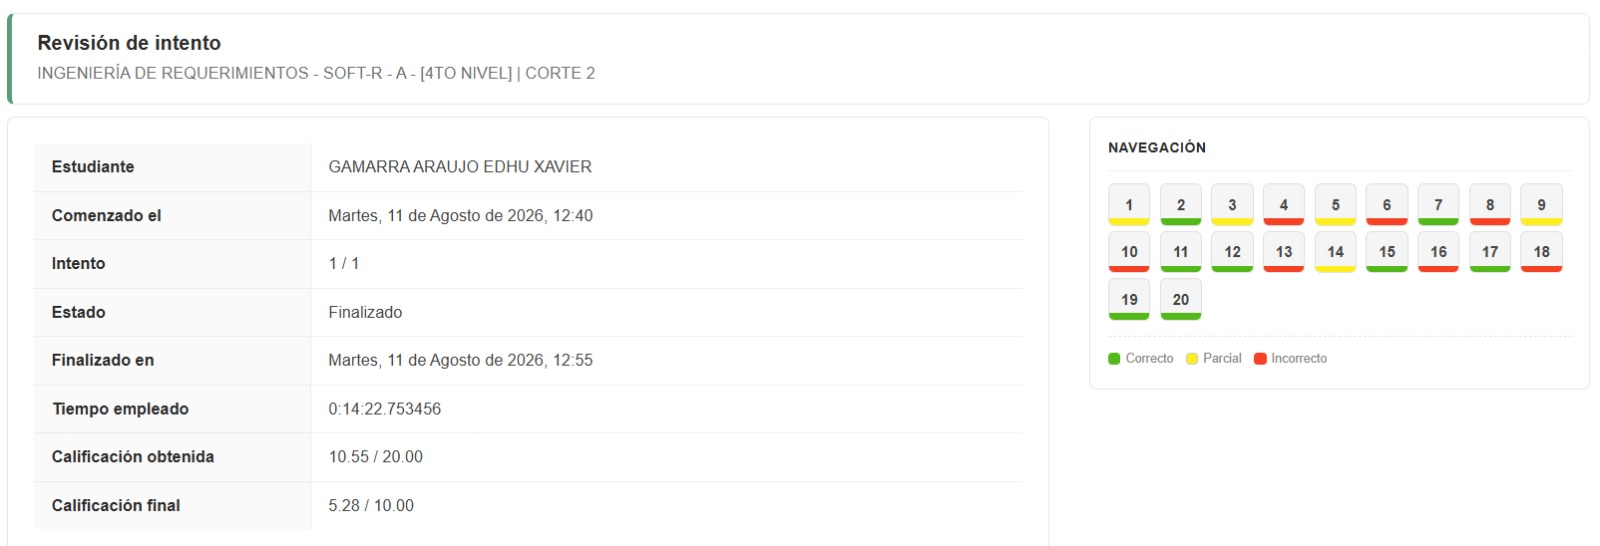
\includegraphics[width=\textwidth]{figuras/CapturaFormativa.jpeg}\\


% GitHub link
{\large \textbf{LINK DE GITHUB:}}\\[0.2cm]
{\large \url{https://github.com/EdhuXav/Gamarra_ISR401_Evaluacion_U4}}

\vfill
\end{titlepage}

\newpage

% ═════════════════════════════════════════════════════════════════════════════
\section{P1. Modelo de datos — Diagrama de clases UML}
% ═════════════════════════════════════════════════════════════════════════════
\begin{figure}[H]
    \centering
    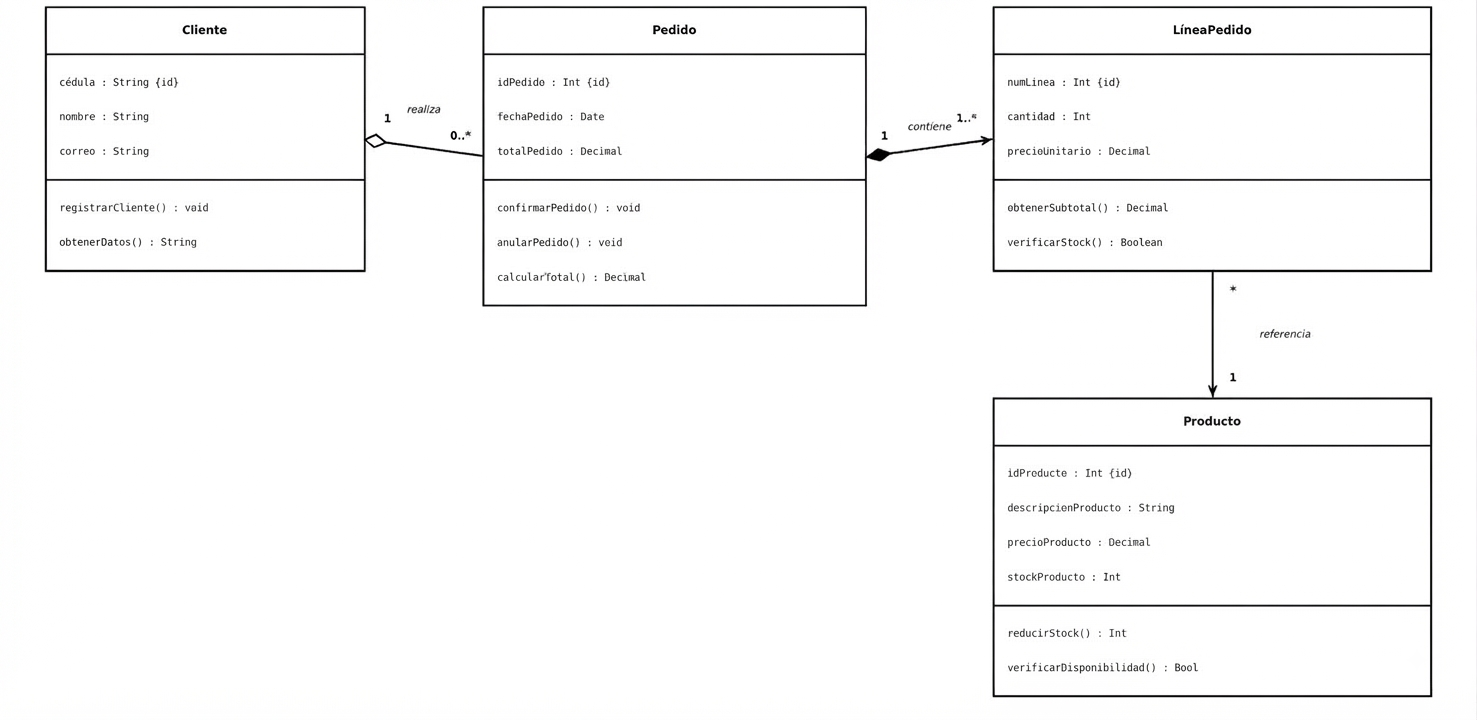
\includegraphics[width=1.1\textwidth,keepaspectratio]{figuras/Diagrama_Clases.png}
    \label{fig:diagrama_clases}
\end{figure}

% ═════════════════════════════════════════════════════════════════════════════
\section{P2. Modelo funcional — Diagrama de actividades UML}
% ═════════════════════════════════════════════════════════════════════════════
\begin{figure}[H]
    \centering
    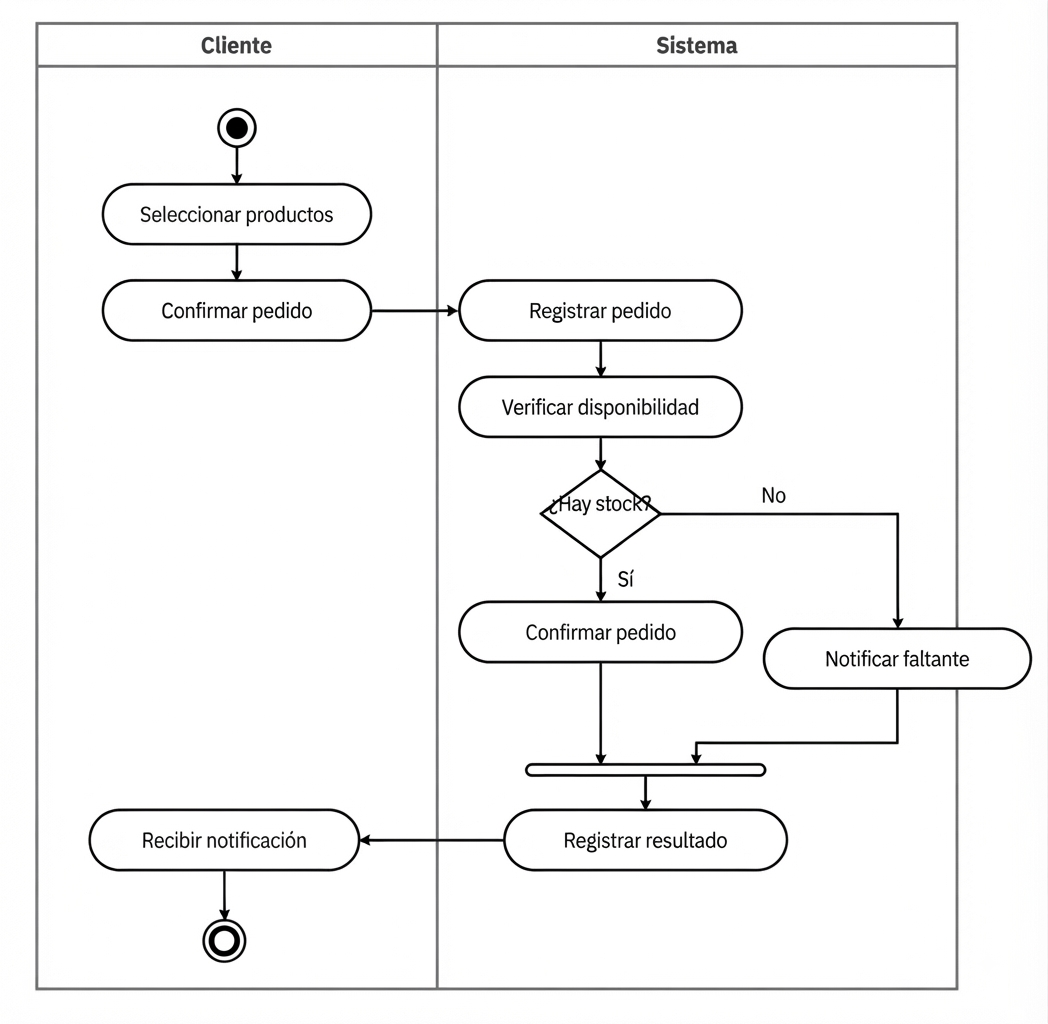
\includegraphics[width=\textwidth,keepaspectratio]{figuras/Diagrama_Actividad.png}
    \label{fig:diagrama_clases}
\end{figure}
\newpage
% ═════════════════════════════════════════════════════════════════════════════
\section{P3. Modelo de comportamiento — Máquina de estados UML}
% ═════════════════════════════════════════════════════════════════════════════
\begin{figure}[H]
    \centering
    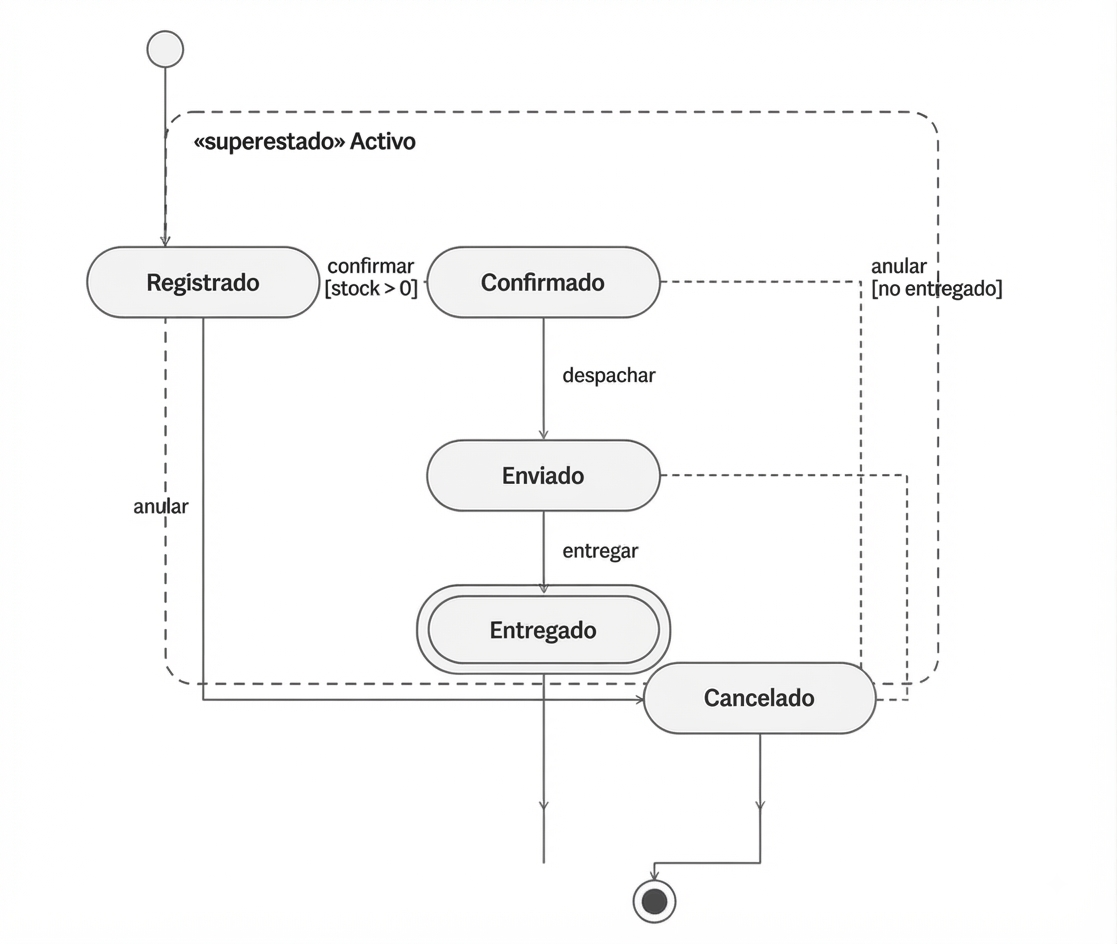
\includegraphics[width=\textwidth,keepaspectratio]{figuras/Diagrama_Estados.png}
    \label{fig:diagrama_clases}
\end{figure}


\newpage
% ═════════════════════════════════════════════════════════════════════════════
\section{P4. Consistencia entre las tres perspectivas}
% ═════════════════════════════════════════════════════════════════════════════

\subsection{Tabla de verificación cruzada}

\begin{table}[H]
\centering
\small
\setlength{\tabcolsep}{4pt}
\begin{tabular}{|p{2.8cm}|p{3.5cm}|p{4cm}|p{2cm}|}
\hline
\rowcolor{lightblue}
\textbf{Evento (P3)} & \textbf{Función / acción (P2)} & \textbf{Entidad / atributo modificado (P1)} & \textbf{Estado} \\
\hline
confirmar {[}stock$>$0{]}
  & Verificar disponibilidad $\rightarrow$ Confirmar pedido
  & \texttt{Pedido.estado} $\leftarrow$ Confirmado; \texttt{Producto.stock} $\leftarrow$ stock$-$cantidad
  & \cellcolor{lightgreen}$\checkmark$ Consistente \\
\hline
notificar faltante
  & Verificar disponibilidad $\rightarrow$ Notificar faltante
  & \texttt{Pedido.estado} permanece Registrado
  & \cellcolor{lightred}$\times$ Defecto \\
\hline
despachar
  & Sin acción específica en P2
  & \texttt{Pedido.estado} $\leftarrow$ Enviado
  & \cellcolor{lightyellow}Fuera de alcance P2 \\
\hline
entregar
  & Sin acción específica en P2
  & \texttt{Pedido.estado} $\leftarrow$ Entregado
  & \cellcolor{lightyellow}Fuera de alcance P2 \\
\hline
anular {[}no entregado{]}
  & Sin acción explícita en P2
  & \texttt{Pedido.estado} $\leftarrow$ Cancelado; \texttt{Producto.stock} $\leftarrow$ stock$+$cantidad
  & \cellcolor{lightyellow}Fuera de alcance P2 \\
\hline
registrar pedido
  & Registrar pedido (carril Sistema)
  & \texttt{Pedido} nueva instancia; \texttt{LíneaPedido} líneas creadas
  & \cellcolor{lightgreen}$\checkmark$ Consistente \\
\hline
\end{tabular}
\end{table}



% ═════════════════════════════════════════════════════════════════════════════
\section{P5. Especificación de requisitos con esquema de atributos}
% ═════════════════════════════════════════════════════════════════════════════
% ── RF-01 ────────────────────────────────────────────────────────────────────
\begin{tcolorbox}[colback=white, colframe=black, boxrule=0.5pt, sharp corners, 
  title={}, breakable]

\medskip
\begin{tabular}{@{}ll@{}}
\textbf{Identificador:}           & RF-01 \\
\textbf{Prioridad:}               & Alta \\
\textbf{Estado:}                  & Propuesto \\
\textbf{Fuente:}                  & Caso de negocio — tienda en línea \\
\textbf{Estabilidad:}             & Alta \\
\textbf{Versión:}                 & 1.0 \\
\textbf{Método de verificación:}  & Prueba funcional \\
\end{tabular}
\end{tcolorbox}

\medskip

% ── RF-02 ────────────────────────────────────────────────────────────────────
\begin{tcolorbox}[colback=white, colframe=black, boxrule=0.5pt, sharp corners, 
  title={}, breakable]

\medskip
\begin{tabular}{@{}ll@{}}
\textbf{Identificador:}           & RF-02 \\
\textbf{Prioridad:}               & Alta \\
\textbf{Estado:}                  & Propuesto \\
\textbf{Fuente:}                  & Ciclo de vida del Pedido — regla de negocio (P3) \\
\textbf{Estabilidad:}             & Media \\
\textbf{Versión:}                 & 1.0 \\
\textbf{Método de verificación:}  & Prueba funcional \\
\end{tabular}
\end{tcolorbox}

\medskip

% ── RNF-01 ───────────────────────────────────────────────────────────────────
\begin{tcolorbox}[colback=white, colframe=black, boxrule=0.5pt, sharp corners, 
  title={}, breakable]

\medskip
\begin{tabularx}{\linewidth}{@{}l X@{}}
\textbf{Identificador:}                    & RNF-01 \\
\textbf{Característica ISO/IEC 25010:}     & Eficiencia de desempeño — comportamiento temporal \\
\textbf{Métrica:}                          & Alto tiempo de respuesta (ms) en percentil 95 \\
\textbf{Umbral:}                           & $< 3\,000$ ms con 100 usuarios a la vez \\
\textbf{Prioridad:}                        & Alta \\
\textbf{Estado:}                           & Propuesto \\
\textbf{Fuente:}                           & ``registrar pedidos con rapidez'' \\
\textbf{Estabilidad:}                      & Media \\
\textbf{Versión:}                          & 1.0 \\
\textbf{Método de verificación:}           & Prueba de rendimiento \\
\end{tabularx}
\end{tcolorbox}

% ── RNF-02 ───────────────────────────────────────────────────────────────────
\begin{tcolorbox}[colback=white, colframe=black, boxrule=0.5pt, sharp corners, 
  title={}, breakable]

\medskip
\begin{tabular}{@{}ll@{}}
\textbf{Identificador:}                    & RNF-02 \\
\textbf{Característica ISO/IEC 25010:}     & Seguridad — confidencialidad \\
\textbf{Métrica:}                          & \% datos personales cifrados \\
\textbf{Umbral:}                           & 100\% de atributos personales cifrados \\
\textbf{Prioridad:}                        & Alta \\
\textbf{Estado:}                           & Propuesto \\
\textbf{Fuente:}                           & ``proteger datos personales de clientes'' \\
\textbf{Estabilidad:}                      & Alta \\
\textbf{Versión:}                          & 1.0 \\
\textbf{Método de verificación:}           & Auditoría de seguridad \\
\end{tabular}
\end{tcolorbox}
% ═════════════════════════════════════════════════════════════════════════════
\section{P6. Priorización MoSCoW}
% ═════════════════════════════════════════════════════════════════════════════

\begin{table}[H]
\centering
\small
\begin{tabular}{|p{3.2cm}|p{2.2cm}|p{2.5cm}|p{5cm}|}
\hline
\rowcolor{lightblue}
\textbf{Requisito} & \textbf{Tipo} & \textbf{Categoría MoSCoW} & \textbf{Valor de negocio} \\
\hline
RF-01 — Registro de pedido
  & Funcional
  & \cellcolor{lightred}\textbf{Must have}
  & Muy alto — Función central \\
\hline
RF-02 — Anulación de pedidos
  & Funcional
  & \cellcolor{lightyellow}\textbf{Should have}
  & Alta — evita errores operativos \\
\hline
RNF-01 — Desempeño $<$3s
  & No Funcional
  & \cellcolor{lightgreen}\textbf{Could have}
  & Medio — mejora experiencia \\
\hline
RNF-02 — Confidencialidad
  & No Funcional
  & \cellcolor{lightred}\textbf{Must have}
  & Muy alto — obligación legal \\
\hline
\end{tabular}
\end{table}



% ═════════════════════════════════════════════════════════════════════════════
\section{P7. Validación por inspección (lista de comprobación 29148)}
% ═════════════════════════════════════════════════════════════════════════════

\begin{table}[H]
\centering
\small
\setlength{\tabcolsep}{4pt}
\begin{tabular}{|p{3.8cm}|p{1.8cm}|p{1.8cm}|p{1.8cm}|p{1.8cm}|}
\hline
\rowcolor{lightblue}
\textbf{Propiedad 29148} & \textbf{RF-01} & \textbf{RF-02} & \textbf{RNF-01} & \textbf{RNF-02} \\
\hline
No ambiguo — único significado posible
  & \cellcolor{lightyellow}Parcial
  & \cellcolor{lightgreen}$\checkmark$ ok
  & \cellcolor{lightgreen}$\checkmark$ ok
  & \cellcolor{lightgreen}$\checkmark$ ok \\
\hline
Completo — toda información necesaria presente
  & \cellcolor{lightred}Falla
  & \cellcolor{lightyellow}Parcial
  & \cellcolor{lightgreen}$\checkmark$ ok
  & \cellcolor{lightgreen}$\checkmark$ ok \\
\hline
Singular — expresa un solo requisito
  & \cellcolor{lightgreen}$\checkmark$ ok
  & \cellcolor{lightgreen}$\checkmark$ ok
  & \cellcolor{lightgreen}$\checkmark$ ok
  & \cellcolor{lightgreen}$\checkmark$ ok \\
\hline
Verificable
  & \cellcolor{lightyellow}Parcial
  & \cellcolor{lightgreen}$\checkmark$ ok
  & \cellcolor{lightgreen}$\checkmark$ ok
  & \cellcolor{lightgreen}$\checkmark$ ok \\
\hline
Factible
  & \cellcolor{lightgreen}$\checkmark$ ok
  & \cellcolor{lightgreen}$\checkmark$ ok
  & \cellcolor{lightyellow}Parcial
  & \cellcolor{lightgreen}$\checkmark$ ok \\
\hline
\end{tabular}
\end{table}

 \newpage
% ═════════════════════════════════════════════════════════════════════════════
\section{P8. Pruebas de aceptación trazadas}
% ═════════════════════════════════════════════════════════════════════════════

\textbf{PA-01: Registro de pedido con stock disponible}
\vspace{0.2cm}


% ── PA-01 ────────────────────────────────────────────────────────────────────
\begin{tcolorbox}[colback=white, colframe=black, boxrule=0.5pt, sharp corners, 
  title={}, breakable]

\medskip
\begin{tabularx}{\linewidth}{@{}l X@{}}
\textbf{Traza:}              & RF-01 — Registro de pedido (versión corregida P7) \\
\textbf{Precondición:}       & Cliente autenticado cédula 0912345678. Producto P-001 stock=10, precio=\$25,00. Producto P-002 stock=5, precio=\$40,00. \\
\textbf{Entradas:}           & Cliente selecciona P-001 (cantidad 2) y P-002 (cantidad 1). Confirma el pedido. \\
\textbf{Pasos ejecución:}    & 1. Iniciar sesión como cliente. 2. Agregar líneas al pedido. 3. Enviar solicitud de registro. 4. Observar respuesta del sistema. \\
\textbf{Criterio de éxito:}  & Sistema crea Pedido en estado \textit{Confirmado}, total=\$90,00; stock de P-001 queda en 8, P-002 en 4. Tiempo de respuesta $\leq 3\,000$ ms. \\
\textbf{Criterio de fallo:}  & Estado distinto de Confirmado, total incorrecto, stock no decrementado o tiempo $> 3\,000$ ms. \\
\end{tabularx}
\end{tcolorbox}


\vspace{0.8cm}
\textbf{PA-02: Anulación de pedido}
\vspace{0.2cm}



% ── PA-02 ────────────────────────────────────────────────────────────────────
\begin{tcolorbox}[colback=white, colframe=black, boxrule=0.5pt, sharp corners, 
  title={}, breakable]

\medskip
\begin{tabularx}{\linewidth}{@{}l X@{}}
\textbf{Traza:}              & RF-02 — Anulación del pedido \\
\textbf{Precondición:}       & Pedido PED-042 en estado Confirmado, creado hace 2 horas, con LíneaPedido: P-001 cantidad 3. Stock actual de P-001 = 7. \\
\textbf{Entradas:}           & Cliente propietario solicita anular PED-042 dentro del plazo de 24 horas. \\
\textbf{Pasos ejecución:}    & 1. Autenticar como Cliente propietario. 2. Seleccionar PED-042. 3. Ejecutar acción ``Anular pedido''. 4. Confirmar la operación. \\
\textbf{Criterio de éxito:}  & PED-042 cambia a estado \textit{Cancelado}. Stock de P-001 se restaura a 10 (7+3). El sistema emite confirmación de anulación al cliente. \\
\textbf{Criterio de fallo:}  & Estado no cambia, stock no se restaura, o anulación permitida fuera del rango de 24h. \\
\end{tabularx}
\end{tcolorbox}


\vspace{0.8cm}
\textbf{PA-03: Tiempo de respuesta bajo carga - registro de pedido}
\vspace{0.2cm}


% ── PA-03 ────────────────────────────────────────────────────────────────────
\begin{tcolorbox}[colback=white, colframe=black, boxrule=0.5pt, sharp corners, 
  title={}, breakable]

\medskip
\begin{tabularx}{\linewidth}{@{}l X@{}}
\textbf{Traza:}              & RNF-01 — Eficiencia de desempeño \\
\textbf{Precondición:}       & Entorno de pruebas con datos de 1000 productos y 500 clientes precargados. Herramienta JMeter configurada con 50 hilos virtuales. \\
\textbf{Entradas:}           & 50 usuarios concurrentes envían solicitudes de registro de pedido. \\
\textbf{Pasos ejecución:}    & 1. Iniciar el plan de prueba JMeter. 2. Ejecutar 10 min de carga sostenida. 3. Recolectar cargas de latencia. 4. Calcular percentil 95. \\
\textbf{Criterio de éxito:}  & Latencia en percentil 95 $\leq 3\,000$ ms. Tasa de error $< 1\%$. Ningún timeout reportado. \\
\textbf{Criterio de fallo:}  & p95 $> 3\,000$ ms, tasa error $\geq 1\%$, o al menos un timeout durante la prueba. \\
\end{tabularx}
\end{tcolorbox}

\newpage
\vspace{0.8cm}
\textbf{PA-04: 
Confidencialidad de datos personales en tránsito y en reposo}
\vspace{0.2cm}

% ── PA-04 ────────────────────────────────────────────────────────────────────
\begin{tcolorbox}[colback=white, colframe=black, boxrule=0.5pt, sharp corners, 
  title={}, breakable]

\medskip
\begin{tabularx}{\linewidth}{@{}l X@{}}
\textbf{Traza:}              & RNF-02 — Seguridad — confidencialidad \\
\textbf{Precondición:}       & Sistema desplegado en entorno de staging. Cliente con datos: cédula 0912345678, nombre ``Ana Torres'', correo ana@example.com registrado. \\
\textbf{Entradas:}           & (a) Captura de tráfico HTTP durante registro. (b) Consulta directa a tabla Cliente en la base de datos. \\
\textbf{Pasos ejecución:}    & 1. Capturar tráfico con Wireshark durante el registro del cliente. 2. Verificar protocolo TLS versión mínima 1.2. 3. Consultar BD y verificar que cédula, nombre y correo aparecen cifrados. 4. Verificar configuración AES-256 en el motor de BD. \\
\textbf{Criterio de éxito:}  & Tráfico capturado muestra TLS $\geq$ 1.2 y cuerpo ilegible. Consulta a BD devuelve atributos cifrados. Configuración AES-256 confirmada. \\
\textbf{Criterio de fallo:}  & Cualquier atributo personal visible en texto plano en tráfico o en BD, o versión TLS inferior a 1.2. \\
\end{tabularx}
\end{tcolorbox}
\newpage


\end{document}
